% ============================================================
% CHAPTER 4: CNN - CONVOLUTIONAL NEURAL NETWORK
% ============================================================
\chapter{Convolutional Neural Network (CNN)}

\section{CNN Theory}

\subsection{Architecture Overview}

CNN is a neural network architecture specifically designed for grid-like structured data (such as images). CNN exploits three key ideas:

\begin{tcolorbox}[colback=blue!5!white,colframe=blue!75!black,title=Three Inductive Biases of CNN]
\begin{enumerate}
    \item \textbf{Locality (Local Receptive Field):} Nearby pixels are more related than distant pixels
    \item \textbf{Translation Equivariance:} A pattern in the top-left corner is also detected in the bottom-right
    \item \textbf{Hierarchy:} Low-level features (edges) → mid-level (shapes) → high-level (objects)
\end{enumerate}
\end{tcolorbox}

\subsection{Convolution Operation}

\subsubsection{Mathematical Definition}

Given input $X \in \mathbb{R}^{H \times W \times C_{in}}$ and kernel $K \in \mathbb{R}^{k \times k \times C_{in} \times C_{out}}$:

\begin{equation}
Y[i,j,c_{out}] = \sum_{m=0}^{k-1} \sum_{n=0}^{k-1} \sum_{c=0}^{C_{in}-1} X[i+m, j+n, c] \cdot K[m, n, c, c_{out}] + b[c_{out}]
\end{equation}

\begin{figure}[H]
\centering
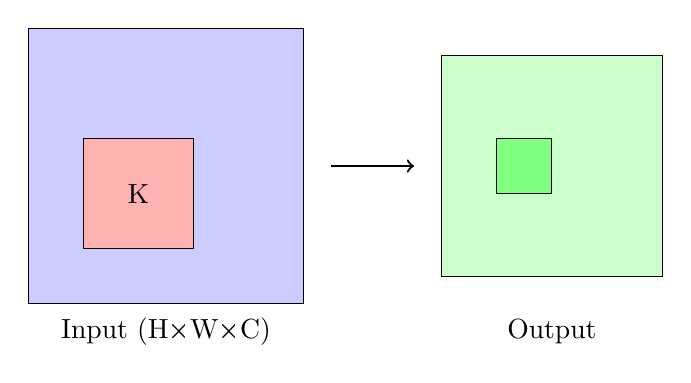
\begin{tikzpicture}[scale=0.7]
    % Input feature map
    \draw[fill=blue!20] (0,0) rectangle (5,5);
    \node at (2.5, -0.5) {Input (H×W×C)};
    
    % Kernel
    \draw[fill=red!30] (1,1) rectangle (3,3);
    \node at (2, 2) {K};
    
    % Arrow
    \draw[->, thick] (5.5, 2.5) -- (7, 2.5);
    
    % Output
    \draw[fill=green!20] (7.5,0.5) rectangle (11.5,4.5);
    \node at (9.5, -0.5) {Output};
    \draw[fill=green!50] (8.5, 2) rectangle (9.5, 3);
\end{tikzpicture}
\caption{Convolution operation: Kernel slides over input}
\end{figure}

\subsubsection{Number of Parameters}

\begin{equation}
\text{Params} = (k \times k \times C_{in} + 1) \times C_{out}
\end{equation}

\textbf{Example:} Conv2d(3, 32, kernel\_size=3):
\begin{equation}
\text{Params} = (3 \times 3 \times 3 + 1) \times 32 = 28 \times 32 = 896
\end{equation}

\subsection{Pooling Layer}

\paperref{Section 3.1 - CNN}

\begin{tcolorbox}[colback=yellow!5!white,colframe=yellow!75!black,title=Paper Quote - Max Pooling]
\textit{``Our CNN Architecture comprises a sequential stack of convolutional layers, accompanied by max pooling layers to reduce spatial dimensions.''}
\end{tcolorbox}

\subsubsection{Max Pooling}

\begin{equation}
Y[i,j] = \max_{(m,n) \in R_{i,j}} X[m,n]
\end{equation}

Where $R_{i,j}$ is the pooling region at position $(i,j)$.

\begin{figure}[H]
\centering
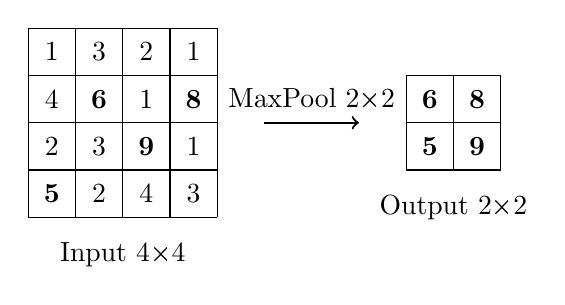
\begin{tikzpicture}[scale=0.6]
    % Input
    \draw (0,0) grid (4,4);
    \node at (0.5, 3.5) {1};
    \node at (1.5, 3.5) {3};
    \node at (2.5, 3.5) {2};
    \node at (3.5, 3.5) {1};
    
    \node at (0.5, 2.5) {4};
    \node at (1.5, 2.5) {\textbf{6}};
    \node at (2.5, 2.5) {1};
    \node at (3.5, 2.5) {\textbf{8}};
    
    \node at (0.5, 1.5) {2};
    \node at (1.5, 1.5) {3};
    \node at (2.5, 1.5) {\textbf{9}};
    \node at (3.5, 1.5) {1};
    
    \node at (0.5, 0.5) {\textbf{5}};
    \node at (1.5, 0.5) {2};
    \node at (2.5, 0.5) {4};
    \node at (3.5, 0.5) {3};
    
    \node at (2, -0.8) {Input 4×4};
    
    % Arrow
    \draw[->, thick] (5, 2) -- (7, 2);
    \node at (6, 2.5) {MaxPool 2×2};
    
    % Output
    \draw (8,1) grid (10,3);
    \node at (8.5, 2.5) {\textbf{6}};
    \node at (9.5, 2.5) {\textbf{8}};
    \node at (8.5, 1.5) {\textbf{5}};
    \node at (9.5, 1.5) {\textbf{9}};
    
    \node at (9, 0.2) {Output 2×2};
\end{tikzpicture}
\caption{Max Pooling 2×2 with stride 2}
\end{figure}

\subsubsection{Benefits of Pooling}

\begin{itemize}
    \item \textbf{Reduces spatial dimensions} → Reduces computation
    \item \textbf{Translation invariance} (slight) → Robust to small shifts
    \item \textbf{Increases receptive field} → Each neuron ``sees'' a wider region
\end{itemize}

\section{CNN Architecture in Paper}

\paperref{Section 3.1 - CNN}

\subsection{Paper Description}

\begin{tcolorbox}[colback=yellow!5!white,colframe=yellow!75!black,title=Paper Quote - CNN Architecture]
\textit{``Our CNN Architecture comprises a sequential stack of convolutional layers, accompanied by max pooling layers to reduce spatial dimensions. We implement dropout to mitigate overfitting. The structure includes a convolution layer with 32 3×3 filters, a max pooling layer with a pool size of 2×2, a convolution layer with 64 3×3 filters, and a max pooling layer with a pool size of 2×2. This is followed by a flatten layer, a dense layer with 512 units and ReLU activation, dropout of 0.5, and an output dense layer with 15 units and softmax activation.''}
\end{tcolorbox}

\subsection{Architecture Diagram}

\begin{figure}[H]
\centering
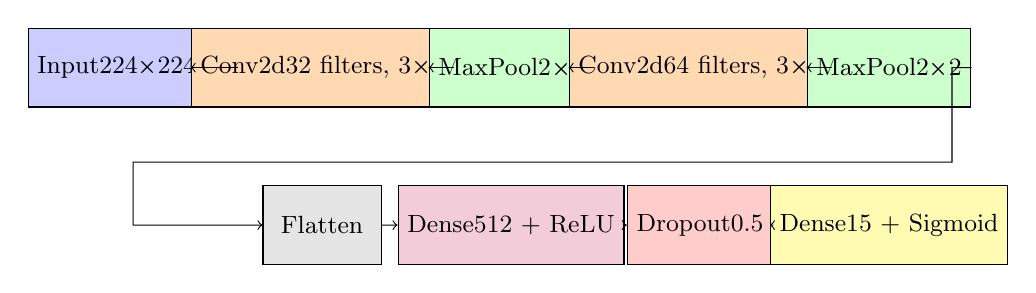
\begin{tikzpicture}[scale=0.8, every node/.style={font=\small}]
    % Input
    \node[draw, fill=blue!20, minimum width=2cm, minimum height=1cm] (input) at (0,0) {Input\\224×224×3};
    
    % Conv1
    \node[draw, fill=orange!30, minimum width=2cm, minimum height=1cm] (conv1) at (3,0) {Conv2d\\32 filters, 3×3};
    
    % Pool1
    \node[draw, fill=green!20, minimum width=1.5cm, minimum height=1cm] (pool1) at (6,0) {MaxPool\\2×2};
    
    % Conv2
    \node[draw, fill=orange!30, minimum width=2cm, minimum height=1cm] (conv2) at (9,0) {Conv2d\\64 filters, 3×3};
    
    % Pool2
    \node[draw, fill=green!20, minimum width=1.5cm, minimum height=1cm] (pool2) at (12,0) {MaxPool\\2×2};
    
    % Flatten
    \node[draw, fill=gray!20, minimum width=1.5cm, minimum height=1cm] (flatten) at (3,-2.5) {Flatten};
    
    % Dense1
    \node[draw, fill=purple!20, minimum width=2cm, minimum height=1cm] (dense1) at (6,-2.5) {Dense\\512 + ReLU};
    
    % Dropout
    \node[draw, fill=red!20, minimum width=1.5cm, minimum height=1cm] (dropout) at (9,-2.5) {Dropout\\0.5};
    
    % Output
    \node[draw, fill=yellow!30, minimum width=2cm, minimum height=1cm] (output) at (12,-2.5) {Dense\\15 + Sigmoid};
    
    % Arrows
    \draw[->] (input) -- (conv1);
    \draw[->] (conv1) -- (pool1);
    \draw[->] (pool1) -- (conv2);
    \draw[->] (conv2) -- (pool2);
    \draw[->] (pool2) -- (13,0) -- (13,-1.5) -- (0,-1.5) -- (0,-2.5) -- (flatten);
    \draw[->] (flatten) -- (dense1);
    \draw[->] (dense1) -- (dropout);
    \draw[->] (dropout) -- (output);
\end{tikzpicture}
\caption{CNN Architecture from paper}
\end{figure}

\section{Mapping Paper → Code}

\coderef{cnn.ipynb}

\subsection{CNN Class Implementation}

\begin{lstlisting}[caption={CNNClassifier in cnn.ipynb (PyTorch)}]
class CNNClassifier(nn.Module):
    def __init__(self, num_classes=15, image_size=224):
        super(CNNClassifier, self).__init__()
        
        # ===== CONVOLUTIONAL LAYERS =====
        # Paper: "convolution layer with 32 3x3 filters"
        self.conv1 = nn.Conv2d(
            in_channels=3,      # RGB input
            out_channels=32,    # 32 filters (from paper)
            kernel_size=3,      # 3x3 kernel (from paper)
            padding=1           # Same padding
        )
        
        # Paper: "max pooling layer with a pool size of 2x2"
        self.pool = nn.MaxPool2d(kernel_size=2, stride=2)
        
        # Paper: "convolution layer with 64 3x3 filters"
        self.conv2 = nn.Conv2d(
            in_channels=32,     # From conv1
            out_channels=64,    # 64 filters (from paper)
            kernel_size=3,      # 3x3 kernel (from paper)
            padding=1
        )
        
        # ===== FULLY CONNECTED LAYERS =====
        # Calculate flatten size after convolutions
        # 224 -> pool -> 112 -> pool -> 56
        # But with valid padding: 224 -> 222 -> 111 -> 109 -> 54
        self.flatten_size = self._get_flatten_size(image_size)
        
        # Paper: "dense layer with 512 units and ReLU activation"
        self.fc1 = nn.Linear(self.flatten_size, 512)
        
        # Paper: "dropout of 0.5"
        self.dropout = nn.Dropout(p=0.5)
        
        # Paper: "output dense layer with 15 units"
        self.fc2 = nn.Linear(512, num_classes)
        
    def _get_flatten_size(self, size):
        """Calculate feature map size after conv layers"""
        # Conv1: (size - 3 + 2*1)/1 + 1 = size (same padding)
        # Pool1: size // 2
        # Conv2: size (same padding)
        # Pool2: size // 2
        size = size // 2  # After pool1
        size = size // 2  # After pool2
        return 64 * size * size  # 64 channels * spatial dims
    
    def forward(self, x):
        # Conv1 + ReLU + Pool
        x = self.pool(F.relu(self.conv1(x)))
        
        # Conv2 + ReLU + Pool
        x = self.pool(F.relu(self.conv2(x)))
        
        # Flatten
        x = x.view(x.size(0), -1)
        
        # FC1 + ReLU + Dropout
        x = self.dropout(F.relu(self.fc1(x)))
        
        # FC2 (no activation - raw logits for BCEWithLogitsLoss)
        x = self.fc2(x)
        
        return x
\end{lstlisting}

\subsection{Detailed Mapping}

\begin{table}[H]
\centering
\caption{Mapping Paper Description → PyTorch Code}
\begin{tabular}{p{5cm}p{5cm}p{3cm}}
\toprule
\textbf{Paper Description} & \textbf{PyTorch Code} & \textbf{Output Shape} \\
\midrule
``convolution layer with 32 3×3 filters'' & \texttt{nn.Conv2d(3, 32, 3, padding=1)} & (B, 32, 224, 224) \\
``max pooling layer 2×2'' & \texttt{nn.MaxPool2d(2, 2)} & (B, 32, 112, 112) \\
``convolution layer with 64 3×3 filters'' & \texttt{nn.Conv2d(32, 64, 3, padding=1)} & (B, 64, 112, 112) \\
``max pooling layer 2×2'' & \texttt{nn.MaxPool2d(2, 2)} & (B, 64, 56, 56) \\
``flatten layer'' & \texttt{x.view(x.size(0), -1)} & (B, 200704) \\
``dense layer with 512 units'' & \texttt{nn.Linear(200704, 512)} & (B, 512) \\
``dropout of 0.5'' & \texttt{nn.Dropout(0.5)} & (B, 512) \\
``output dense layer with 15 units'' & \texttt{nn.Linear(512, 15)} & (B, 15) \\
\bottomrule
\end{tabular}
\end{table}

\section{Detailed Layer Analysis}

\subsection{Layer 1: Conv2d(3, 32, 3)}

\begin{tcolorbox}[colback=blue!5!white,colframe=blue!75!black,title=Analysis: First Convolution Layer]
\textbf{Purpose:} Extract low-level features (edges, gradients, textures)

\textbf{Input:} 224 × 224 × 3 (RGB image)

\textbf{Operation:}
\begin{itemize}
    \item 32 learnable kernels, each 3×3×3
    \item Slide over input with stride 1
    \item With padding=1: output same spatial size
\end{itemize}

\textbf{Parameters:}
\begin{equation}
(3 \times 3 \times 3 + 1) \times 32 = 896 \text{ parameters}
\end{equation}

\textbf{Output:} 224 × 224 × 32
\end{tcolorbox}

\subsection{Layer 2-3: MaxPool → Conv2d(32, 64, 3)}

\begin{tcolorbox}[colback=green!5!white,colframe=green!75!black,title=Analysis: Second Stage]
\textbf{MaxPool2d(2, 2):}
\begin{itemize}
    \item Reduces spatial size: 224 → 112
    \item No learnable parameters
    \item Adds translation invariance
\end{itemize}

\textbf{Conv2d(32, 64, 3):}
\begin{itemize}
    \item Input: 112 × 112 × 32
    \item Learns 64 filters to detect mid-level features
    \item Parameters: $(3 \times 3 \times 32 + 1) \times 64 = 18,496$
    \item Output: 112 × 112 × 64
\end{itemize}
\end{tcolorbox}

\subsection{Flatten + Dense Layers}

\begin{tcolorbox}[colback=purple!5!white,colframe=purple!75!black,title=Analysis: Classification Head]
\textbf{After second pooling:} 56 × 56 × 64 = 200,704 values

\textbf{Dense(200704, 512):}
\begin{itemize}
    \item Largest layer by parameters
    \item Parameters: $200,704 \times 512 + 512 = 102,760,960$
    \item Learns non-local relationships
\end{itemize}

\textbf{Dropout(0.5):}
\begin{itemize}
    \item Randomly zeros 50\% of activations during training
    \item Acts as regularization
    \item No parameters
\end{itemize}

\textbf{Dense(512, 15):}
\begin{itemize}
    \item Output layer for 15 classes
    \item Parameters: $512 \times 15 + 15 = 7,695$
\end{itemize}
\end{tcolorbox}

\section{Total Parameters Analysis}

\begin{table}[H]
\centering
\caption{CNN Parameter Count}
\begin{tabular}{lcr}
\toprule
\textbf{Layer} & \textbf{Formula} & \textbf{Parameters} \\
\midrule
Conv1 & $(3 \times 3 \times 3 + 1) \times 32$ & 896 \\
Conv2 & $(3 \times 3 \times 32 + 1) \times 64$ & 18,496 \\
FC1 & $200,704 \times 512 + 512$ & 102,760,960 \\
FC2 & $512 \times 15 + 15$ & 7,695 \\
\midrule
\textbf{Total} & & \textbf{102,788,047} \\
\bottomrule
\end{tabular}
\end{table}

\begin{tcolorbox}[colback=red!5!white,colframe=red!75!black,title=Observation]
\textbf{99.97\%} of parameters are in the FC1 layer!

This is a common problem with traditional CNNs: the flatten layer creates too many connections.

\textbf{Solutions:}
\begin{itemize}
    \item Global Average Pooling (instead of flatten)
    \item Add more conv layers to reduce spatial size
    \item Use different architecture (ResNet, ViT)
\end{itemize}
\end{tcolorbox}

\section{Loss Function: BCEWithLogitsLoss}

\subsection{Why Not CrossEntropyLoss?}

\begin{table}[H]
\centering
\begin{tabular}{lcc}
\toprule
\textbf{Aspect} & \textbf{CrossEntropyLoss} & \textbf{BCEWithLogitsLoss} \\
\midrule
Task type & Multi-class (one-hot) & Multi-label (independent) \\
Output activation & Softmax & Sigmoid (per class) \\
Sums to 1? & Yes & No \\
NIH dataset & \textcolor{red}{\ding{55}} & \textcolor{green}{\ding{51}} \\
\bottomrule
\end{tabular}
\end{table}

\subsection{BCEWithLogitsLoss Formula}

\begin{equation}
\mathcal{L} = -\frac{1}{N \times C} \sum_{i=1}^{N} \sum_{c=1}^{C} \left[ y_{i,c} \log(\sigma(z_{i,c})) + (1-y_{i,c}) \log(1-\sigma(z_{i,c})) \right]
\end{equation}

Where:
\begin{itemize}
    \item $\sigma(z) = \frac{1}{1 + e^{-z}}$ (sigmoid function)
    \item $y_{i,c} \in \{0, 1\}$ is ground truth
    \item $z_{i,c}$ is raw logit from model
\end{itemize}

\section{Results and Analysis}

\paperref{Section 5 - Experiments}

\subsection{Paper Results}

\begin{tcolorbox}[colback=yellow!5!white,colframe=yellow!75!black,title=Paper Results - CNN]
\begin{itemize}
    \item \textbf{Training Accuracy:} 91\%
    \item \textbf{Validation AUC:} 0.82
    \item \textbf{Test AUC:} 0.82
\end{itemize}
\end{tcolorbox}

\subsection{Performance Analysis}

\begin{tcolorbox}[colback=blue!5!white,colframe=blue!75!black,title=Analysis: Why CNN Performs Worst?]
\textbf{Reasons why CNN has the lowest performance among 5 models:}

\begin{enumerate}
    \item \textbf{Limited Receptive Field:}
    \begin{itemize}
        \item Only 2 conv layers
        \item Small receptive field, hard to capture global features
        \item X-ray pathologies can span the entire image
    \end{itemize}
    
    \item \textbf{No Skip Connections:}
    \begin{itemize}
        \item Gradient must flow through all layers
        \item May suffer from vanishing gradient
        \item Difficult to train deeper variants
    \end{itemize}
    
    \item \textbf{Overfitting Risk:}
    \begin{itemize}
        \item >100M parameters, mostly from FC layer
        \item Dataset of 85K images may not be enough
        \item Despite having dropout 0.5
    \end{itemize}
\end{enumerate}
\end{tcolorbox}

\section{Comparison with Other Architectures}

\begin{table}[H]
\centering
\caption{CNN vs ResNet vs ViT}
\begin{tabular}{lccc}
\toprule
\textbf{Aspect} & \textbf{CNN} & \textbf{ResNet} & \textbf{ViT} \\
\midrule
Depth & 4 layers & 34 layers & 8 blocks \\
Skip connections & No & Yes & No (but attention) \\
Inductive bias & Strong (locality) & Strong & Weak \\
Global context & Poor & Medium & Excellent \\
Parameters & 102M & 21M & 3M \\
Training accuracy & 91\% & 93\% & 93.9\% \\
\bottomrule
\end{tabular}
\end{table}
